\section{Methodology}
\label{sec:methodology}

\subsection{Overview}
\label{subsec:method-overview}

\textsc{Trident} models each positioning trajectory as a recursive scan over $N$ sensor samples. At step $k$, the scan reads the current IMU and odometer measurements, propagates the nominal SINS state, performs EKF prediction and correction, feeds the estimated error back to the nominal state, and carries the updated navigation state and covariance to step $k+1$. A batch of $B$ simulations adds an outer trajectory dimension to the input and output tensors; the recurrent state remains private to each trajectory.

\Cref{fig:design-overview} summarizes three complementary optimizations. First, whole-scan fusion encloses the complete time loop in one kernel, retains recurrent state on chip, and specializes the small-matrix operations on the critical path. Second, component-aware precision specialization assigns representations according to numerical role and selects a compile-time precision plan under a trajectory-level error constraint. Third, multi-trajectory mapping assigns independent scans to separate CUDA blocks, exposing device-wide parallelism subject to register-residency limits. The three axes target different bottlenecks---dispatch and data movement, arithmetic and storage cost, and insufficient device-level parallelism---and can therefore be composed.

These transformations preserve the SINS/EKF equations and the order of propagation, measurement selection, prediction, correction, and feedback within every trajectory. We use the CPU fp64 implementation as the semantic reference, compare complete output trajectories rather than isolated steps, and repeat identical trajectories across blocks to detect accidental state sharing. \Cref{sec:evaluation} reports the corresponding performance and accuracy results.

\begin{figure}[!t]
  \centering
  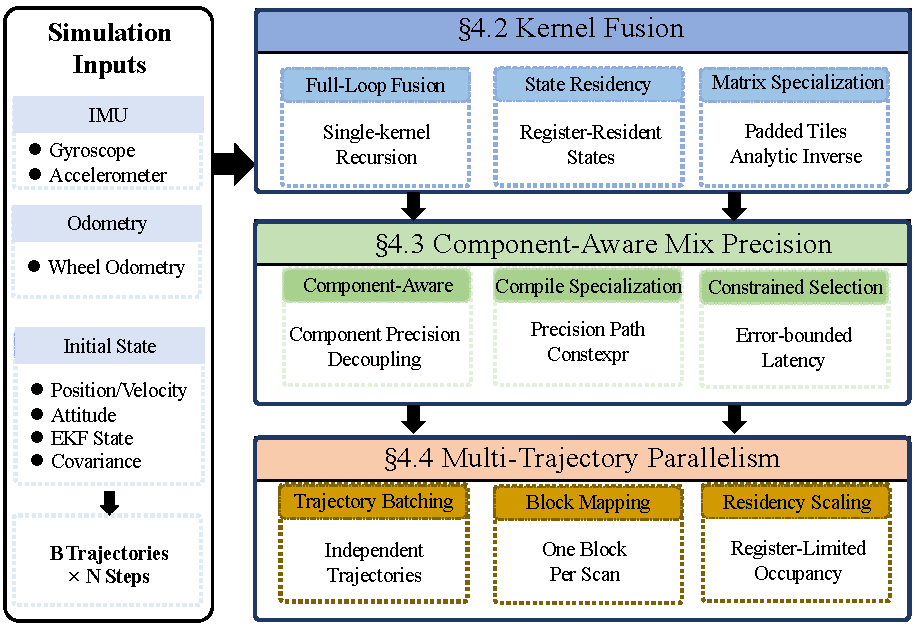
\includegraphics[width=\linewidth]{figures/4-method-overview.pdf}
  \caption{Overview of \textsc{Trident}. Kernel fusion retains recurrent state on chip, component-aware mixed precision selects numerically safe precision paths, and block-level trajectory mapping exposes device-wide parallelism.}
  \label{fig:design-overview}
\end{figure}

\subsection{From Fragmented Operators to a Fused Recursive Scan}
\label{subsec:kernel-fusion}

\Cref{fig:fusion-path}(a) contrasts the eager and whole-scan fusion boundaries. In the eager implementation, one filter step expands into approximately 531 dependent kernels. Recurrent values therefore cross kernel boundaries and return to HBM hundreds of times per step, even though the next operation immediately consumes them.

We first regularize the step for static compilation. Scalar tensor construction, host-visible scalar access, and dynamic concatenation are replaced with device-side expressions. The observation shapes that arise when the consistency test rejects a component are unified into one fixed three-dimensional representation; a large variance suppresses the corresponding Kalman gain without changing the matrix shape. CUDA Graph replay then removes repeated host dispatch, but the captured graph still contains the fine-grained kernels and their recurrent-state transfers. Whole-scan fusion removes this remaining boundary by placing all $N$ steps inside one Triton program. A single host launch enters the scan, and the loop preserves the original update order while reusing state across iterations.

\begin{figure}[!t]
  \centering
  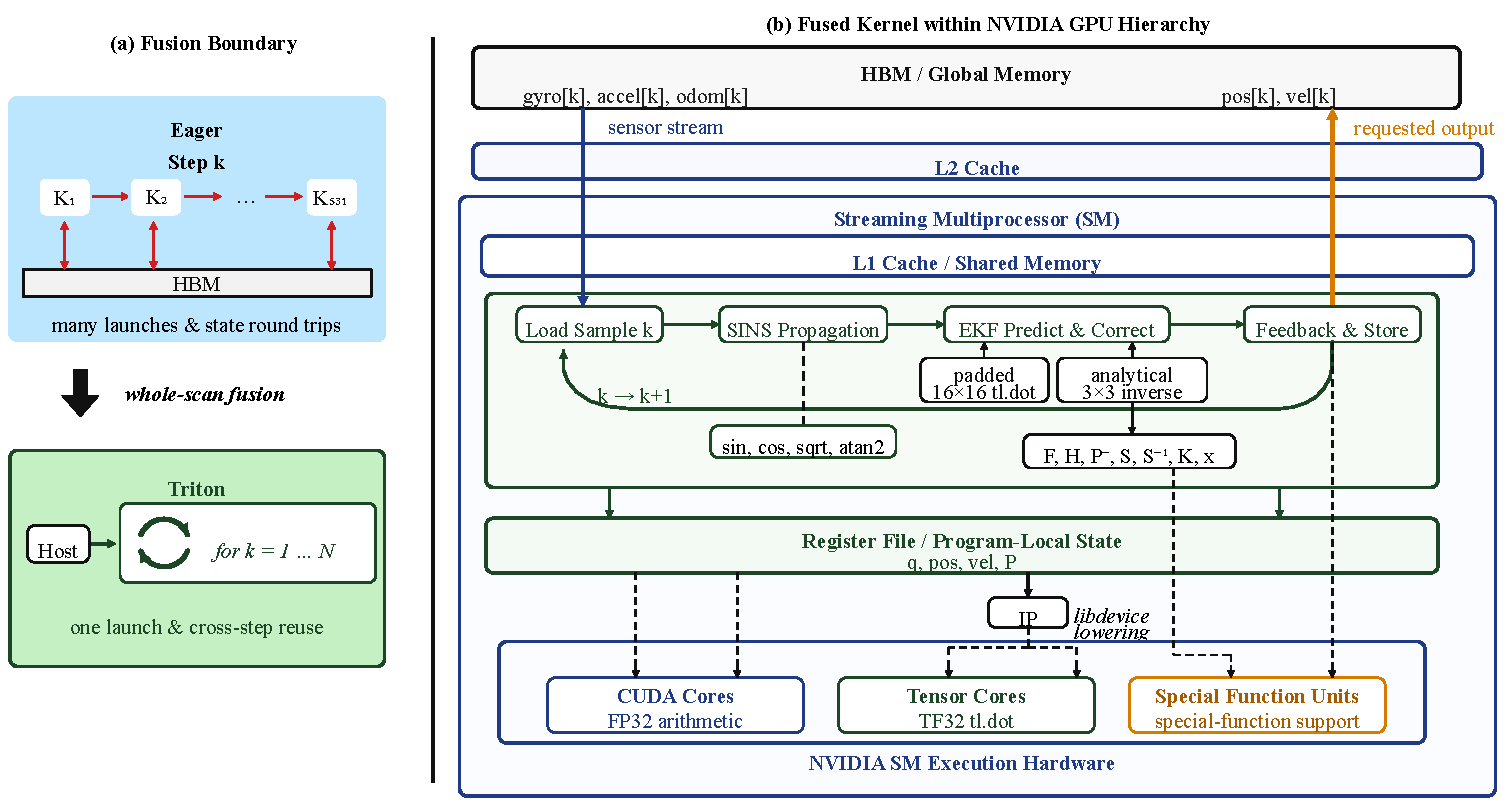
\includegraphics[width=\linewidth]{figures/4-method-fusion.pdf}
  \caption{Whole-scan fusion and its GPU mapping. (a) Fusion replaces hundreds of eager kernels per step with one Triton launch for the full trajectory. (b) The fused program streams sensor samples and requested outputs through HBM while retaining recurrent state in registers and mapping matrix and special-function operations to the corresponding SM execution units.}
  \label{fig:fusion-path}
\end{figure}

\Cref{fig:fusion-path}(b) shows the resulting data path. At iteration $k$, the program streams only the current gyroscope, accelerometer, and odometer samples through L2 and the SM cache hierarchy. It performs SINS propagation, EKF prediction and correction, and feedback before advancing to $k+1$. Only the requested position and velocity outputs are written to global memory. The quaternion, position, velocity, error state, and covariance remain program-local, so the loop-carried dependency passes through the register file instead of intermediate global-memory tensors.

Two in-kernel transformations make the loop static and self-contained. First, masked $16\times16$ tiles store the logical 15-state filter matrices, providing a common layout for transition, covariance, observation, and gain products. The compile-time dot-product mode lowers these products to either CUDA-core IEEE arithmetic or Tensor Core TF32 operations. Second, the kernel computes the inverse of the $3\times3$ innovation covariance from its adjugate and determinant, avoiding a general solver and its synchronization point. SINS transcendental functions, including sine, cosine, square root, and arctangent, follow the device special-function path. The mapping in \Cref{fig:fusion-path}(b) thus combines one fusion boundary, register-resident recurrence, and hardware-specific micro-operations to reduce dispatch, synchronization, and HBM traffic on the latency-bound critical path.

\subsection{Component-Aware Precision Specialization}
\label{subsec:mixed-precision}

Uniform precision ignores the different numerical roles within the scan. Sensor samples are noisy, once-consumed inputs, whereas position, velocity, attitude, error state, and covariance recur across the complete trajectory and can accumulate rounding error. Small matrix products introduce a third choice because TensorFloat-32 (TF32) changes the multiplication path without changing the surrounding storage type. We therefore treat input storage, recurrent arithmetic, and dot-product mode as independent dimensions.

The fused kernel exposes these dimensions as three compile-time parameters. $\mathit{DT}_{\mathrm{IO}}$ specifies the stored type of IMU and odometer samples, which are converted on load to the internal arithmetic type $\mathit{DT}$. The latter governs quaternion normalization, SINS integration, EKF prediction, covariance update, and feedback. $\mathit{IP}$ selects the Triton dot-product mode, distinguishing IEEE and TF32 execution. Because all three parameters are compile-time constants, each combination produces a branch-free specialized kernel. We define a precision plan as $P=(\mathit{DT}_{\mathrm{IO}},\mathit{DT},\mathit{IP})$ over the candidate sets in \Cref{tab:precision-design}. For this workload the plan selected by \Cref{eq:precision-accept} is, as the evaluation reports, the all-fp32/IEEE plan---fp32 sensor input, fp32 recursive arithmetic, and IEEE dot products---while TF32 products are excluded on accuracy and hardware grounds.

\begin{table}[H]
  \centering
  \caption{Precision dimensions exposed by the fused implementation.}
  \label{tab:precision-design}
  \begin{tabular}{@{}lll@{}}
    \toprule
    Component & Candidates & Treatment \\
    \midrule
    Sensor input & fp16, bf16, fp32 & cast to $\mathit{DT}$ \\
    Recursive computation & fp32, fp64 & retain across steps \\
    Small matrix products & IEEE, TF32 & $\mathit{IP}$ specialization \\
    Validation reference & fp64 & CPU trajectory \\
    \bottomrule
  \end{tabular}
\end{table}

We screen each plan over the complete trajectory rather than an isolated filter step. Let $\mathbf{p}^{P}_{0:N}$ be the position trajectory produced by plan $P$, and let $\mathbf{p}^{\mathrm{ref}}_{0:N}$ be the CPU fp64 trajectory. The precision-induced deviation is
\(
  \delta_{P}=\mathrm{RMSE}(\mathbf{p}^{P}_{0:N},\mathbf{p}^{\mathrm{ref}}_{0:N}).
\)
Evaluating all $N$ steps exposes errors that emerge only after repeated integration or covariance propagation. We separately define the irreducible model error as $\varepsilon_{\mathrm{model}}=\mathrm{RMSE}(\mathbf{p}^{\mathrm{ref}}_{0:N},\mathbf{p}^{\mathrm{truth}}_{0:N})$. For a dimensionless tolerance $\alpha$, plan $P$ is acceptable when
\begin{equation}
  \delta_{P}\le\alpha\,\varepsilon_{\mathrm{model}},
  \label{eq:precision-accept}
\end{equation}
so that numerical error introduced by the precision plan remains small relative to the model error already present in the fp64 reference. This criterion separates numerical acceptance from hardware behavior: $\mathit{DT}_{\mathrm{IO}}$ changes input storage and bandwidth, $\mathit{DT}$ changes recurrent arithmetic and state representation, and $\mathit{IP}$ changes dot-product execution. Among the acceptable plans, we select the one with the lowest critical-path latency $\tau_{P}$, breaking ties by the smaller register footprint $r_{P}$. We also retain the nondominated precision--latency set; \Cref{fig:precision-tradeoff} in \Cref{subsec:motivation-precision} plots its throughput--deviation trade-off, and \Cref{subsec:precision-evaluation} evaluates the surviving accuracy ordering. \Cref{alg:precision-selection} summarizes the procedure.

\begin{algorithm}[H]
  \caption{Component-Aware Precision Plan Selection}
  \label{alg:precision-selection}
  \begin{algorithmic}[1]
    \Require
      candidate sets $\Pi_{\mathrm{IO}},\Pi_{\mathrm{R}},\Pi_{\mathrm{dot}}$;
      sensor stream $\mathbf{Z}_{0:N-1}$;
      fp64 position trajectory $\mathbf{p}^{\mathrm{ref}}_{0:N}$;
      model error $\varepsilon_{\mathrm{model}}$;
      acceptance ratio $\alpha$
    \Ensure
      selected plan
      $P^{\star}=(\mathit{DT}_{\mathrm{IO}}^{\star},\mathit{DT}^{\star},\mathit{IP}^{\star})$
      and Pareto front $\mathcal{F}$
    \State $\mathcal{C} \gets \Pi_{\mathrm{IO}} \times \Pi_{\mathrm{R}} \times \Pi_{\mathrm{dot}}$
      \Comment{enumerate component-wise candidates}
    \State $\mathcal{R} \gets \emptyset$
      \Comment{error, latency, and register footprint}
    \ForAll{$P=(\mathit{DT}_{\mathrm{IO}},\mathit{DT},\mathit{IP}) \in \mathcal{C}$}
      \State $K_{P} \gets \textsc{Specialize}(\mathit{DT}_{\mathrm{IO}},\mathit{DT},\mathit{IP})$
        \Comment{compile-time constants; no runtime branch}
      \State $(\mathbf{p}^{P}_{0:N},\tau_{P},r_{P}) \gets \textsc{RunTrajectory}(K_{P},\mathbf{Z}_{0:N-1})$
        \Comment{full $N$-step scan}
      \State $\delta_{P} \gets \mathrm{RMSE}(\mathbf{p}^{P}_{0:N},\mathbf{p}^{\mathrm{ref}}_{0:N})$
        \Comment{trajectory-level deviation}
      \If{$\delta_{P} \le \alpha\,\varepsilon_{\mathrm{model}}$}
        \Comment{accept by \Cref{eq:precision-accept}}
        \State $\mathcal{R} \gets \mathcal{R}\cup\{(P,\delta_{P},\tau_{P},r_{P})\}$
      \EndIf
    \EndFor
    \State $\mathcal{F} \gets \textsc{ParetoFront}(\mathcal{R};\ \text{minimize}\ \delta_{P},\ \text{minimize}\ \tau_{P})$
    \State $P^{\star} \gets \arg\min_{(P,\cdot,\tau_{P},r_{P})\in\mathcal{R}} \tau_{P}$,
      ties broken by smallest $r_{P}$
      \Comment{fastest accepted plan}
    \State \Return $P^{\star},\ \mathcal{F}$
  \end{algorithmic}
\end{algorithm}

\subsection{Multi-Trajectory Batch Parallelism}
\label{subsec:batch-parallelism}

A fused scan for one trajectory occupies one CUDA block, leaving most SMs without useful work. Simulation campaigns, however, naturally contain independent trajectories generated from different noise seeds, obstacle configurations, or filter parameters. Because these trajectories share the same computation but no recurrent state, they provide an outer parallel dimension without altering the sequential scan. For batch size $B$, we launch a one-dimensional grid of $B$ Triton programs and assign trajectory $b$ to program identifier $b$. Suppressing the innermost component offset, each input and output address has the form
\begin{equation}
  \operatorname{addr}(b,k)=\operatorname{base}+b\,s_B+k\,s_N,
  \label{eq:batch-address}
\end{equation}
where $s_B$ and $s_N$ are the trajectory and time strides. Each program initializes its SINS and EKF state independently, so trajectories require neither synchronization nor communication.

This mapping yields a resource-based scaling model. Let $S$ be the number of SMs, $R_{\mathrm{SM}}$ the register capacity of one SM, and $R_{\mathrm{blk}}$ the register allocation of one trajectory block. When registers are the active residency constraint, the number of resident blocks per SM and the corresponding device-wide saturation batch are approximated by
\begin{equation}
  C_{\mathrm{reg}}=\left\lfloor
  \frac{R_{\mathrm{SM}}}{R_{\mathrm{blk}}}\right\rfloor,
  \qquad B_{\mathrm{sat}}\approx S C_{\mathrm{reg}}.
  \label{eq:batch-saturation}
\end{equation}
This approximation omits architectural limits on blocks, warps, shared memory, and scheduling, and therefore serves as a scaling guide rather than an exact occupancy model. For $B\leq S$, trajectories can be distributed across distinct SMs and aggregate throughput should grow nearly linearly. For $S<B\leq B_{\mathrm{sat}}$, additional resident blocks increase contention for registers and execution units. Beyond $B_{\mathrm{sat}}$, blocks execute in waves, so increasing $B$ improves total work capacity but not instantaneous throughput. The batch-size sweep of \Cref{subsec:ablation} (\Cref{tab:ablation-batch}) tests these regimes.

\subsection{Implementation Details}
\label{subsec:implementation-details}

The complete scan is implemented as one \texttt{@triton.jit} kernel with launch grid $(B,)$. Each Triton program owns one trajectory, iterates over its $N$ samples, and accesses fixed-shape state and matrix tiles through masked loads and stores. Precision types, dot-product mode, tile shape, and launch configuration are compile-time meta-parameters; specialization therefore introduces no runtime branch into the recurrent loop. Input and output buffers are allocated before launch, and compilation and autotuning are excluded from measured execution time~\cite{triton}.

On the evaluated Hopper GPU, Triton lowers eligible \texttt{tl.dot} operations to Tensor Core instructions for TF32 plans and uses CUDA-core arithmetic for IEEE plans. Scalar transcendental functions follow the backend's device-library lowering, while the analytical innovation inverse remains inside the program. We use conventional coalesced loads and stores for the per-step sensor stream because the scan consumes only a small sample at each iteration; the large recurrent state remains register-resident rather than being staged repeatedly through shared memory or TMA. This implementation matches the memory and execution mapping in \Cref{fig:fusion-path}(b) while keeping the precision and launch choices explicit~\cite{nvidia2022hopper}.
